%!TEX root = ../Main.tex

% -----------------------------------------------------------------------------
\section{Fusion in Practice}
\label{s:Evaluation}

Stream fusion is ultimately performed for practical reasons. We want the fused result program to run faster than unfused source program. Fused result programs like the one in Fig. \ref{fig:Process:Fused} can be lowered directly to a target language, such as Haskell (maybe using Template Haskell), C or LLVM abstract assembly. The details of such lowering surely affect the performance of the final program, but as they are largely unrelated to the fusion algorithm itself, we focus on the form of the fused program expressed directly in the process language.


% -----------------------------------------------------------------------------
\subsection{Fusability}
\label{s:FusionOrder}
When we fuse a pair of processes we commit to a particular interleaving of instructions from each process. When we have at least three processes to fuse, the choice of which two to handle first can determine whether this fused result can then be fused with the third process. Consider our @alternatives@ example from \S\ref{s:EvaluationOrder}, here it is again:
\begin{code}
  alternates : S Nat -> S Nat -> S Nat -> S (Nat, Nat)
  alternates sInA sInB sInC
   = let  s1   = alt2 sInA sInB
          s2   = alt2 sInB sInC
          sOut = zip s1 s2
     in   sOut
\end{code}

In our current system, if fuse the two @alt2@ processes together first, then try to fuse this result process with the downstream @zip@ process, then this final fusion transform fails. This happens because the first fusion transform commits to a sequential instruction interleaving where two output values \emph{must} be pushed to stream @s1@ first, before then pushing values to @s2@. As we discussed in \S\ref{s:EvaluationOrder}, the downstream @zip@ process needs to pull single values from @s1@ and @s2@ alternatively.

Dynamically, if we were to try to execute the result process and the downstream @zip@ process concurrently, then the execution would deadlock. Statically, when we try to fuse the result process with the downstrem @zip@ process then the deadlock is discovered and fusion fails. Deadlock happens when neither process can advance to the next instruction, and in the fusion algorithm this will manifest as the failure of the $tryStepPair$ function from Fig.\ref{fig:Fusion:Def:StepPair}. The $tryStepPair$ function determines which of the instructions from either process can be executed next, and when execution is deadlocked there are none.

On the upside, fusion failure is easy to detect. It is also easy to provide a report to the client programmer that describes why two particular processes could not be fused. The report is phrased in terms of the process definitions visible to the client programmer, instead of partially fused intermediate code. The joint labels used in the fusion algorithm represent which states each of the original processes would be in during a concurrent execution, and we provide the corresponding instructions as well as the abstract states of all the input channels. This reporting ability is \emph{significantly better} than that of prior fusion systems such as Repa~\cite{lippmeier2012:guiding}, as well as the co-recursive stream fusion of \cite{coutts2007stream}, and may other systems based on general purpose program transformations. In such systems it is usually not clear whether the fusion transformation even succeeded, and debugging why it might not have succeeded involves spelunking\footnote{def. spelunking: Exploration of caves, especially as a hobby. Usually not a science.} through many pages (sometimes hundreds of pages) of compiler intermediate representations.

In practice, the likelihood of fusion suceeding depends on the particular dataflow network being used, as well as the form of the processes in that network. For fusion of pipelines of standard combinators such as @map@, @fold@, @filter@, @scan@ and so on, fusion always succeeds. The process implementations of each of these combinators only pull one element at a time from their source streams, before pushing the result to the output stream, so there is no possiblity of deadlock. Deadlock can only happen when multiple streams fan-in to a process with multiple inputs, such as with @merge@. When the dataflow network has a single output stream then we use the method of starting from the process closes to the output stream, walking to towards the input streams, and fusing in successive processes as they occur. This allows the interleaving of the intermediate fused process to be dominated by the consumers, rather than producers, as consumers are more likely to have multiple input channels which need to be synchronized. In the worst case the fallback approach is to try all possible orderings of processes to fuse, assuming the client programmer is willing to wait for the search to complete. 

% We discuss other possible approaches in \S\ref{s:Future:FusionOrder}. 


% When the two @alt2@ processes are fused we end up with a sequential result process. Trying to then fuse that result into the downstream @zip@ process fails. Alternately, if we were to try to concurrently evaluate the fused result process with the downstream @zip@ process would deadlock because we would reach a state where neither process could advance. To state this again: fusion fails when concurrent evaluation of the two source processes would deadlock.

% The main fusion algorithm here works on pairs of processes.
% When there are more than two processes, there are multiple orders in which the pairs of processes can be fused. The order in which pairs of processes are fused does not affect the output values, but it does affect the access pattern: the order in which outputs are produced and inputs read. Importantly, the access pattern also affects whether fusion succeeds or fails to produce a process. In other words, while evaluating multiple processes is non-deterministic, the act of fusing two processes \emph{commits} to a particular deterministic interleaving of the two processes. The simplest example of this has two input streams, a function applied to both, then zipped together. 



% -----------------------------------------------------------------------------
\subsection{Result Size}

As with fusion transformation system, we must be careful that the size of the result code does not become too large when more and more processes are fused together. The left of Fig.\ref{fig:bench:outputsize} shows the maximum number of output states in the result when a particular number of processes are fused together in a pipelined-manner. To produce this graph we programmatically generated dataflow networks for \emph{all possible} pipelined combinations of the @map@, @filter@, @scan@, @group@ and @merge@ combinators, and tried all possible fusion orders consiting of adjacent pairs of processes. The @merge@ combinator itself has two inputs, so only works at the very start of the pipeline --- we present result for pipelines with and without a @merge@ at the start. The right of Fig.\ref{fig:bench:outputsize} shows the number of states in the result when the various combinations of combinators are fused in parallel, for example, we might have a @map@ and a @filter@ processing the same input stream. In both cases the number of states in the result process grows linearly with the number of processes. In all combinations, with up to 7 processes there are less than 100 states in the result process. 
%%% AR: Note that the split version also has only one merge?

The size of the result process is roughly what one would get when inlining the definitions of each of the original source processes. This is common with other systems based on inlining and/or template meta-programming, and is not prohibitive.

On the other hand, Fig.\ref{fig:bench:exponential} shows the results for a pathological case where the size of the output program is exponential in the number if input processes. The source dataflow networks consists of N merge processes, N+1 input streams, and a single output stream. The output of each merge process is the input of the next, forming a chain of merges. In source notation the network for N = 3 is @sOut = merge sIn1 (merge sIn2 (merge sIn3 sIn4))@.

When fusing two processes the fusion algorithm essentially compares every state in the first process with every state in the second, computing a cross product. During the fusion transform, as states in the result process are generated they are added to a finite map --- the @instrs@ field of the process definition. The use of the finite map ensures that identical states are always combined, but genuinly different states always make it into the result. 

In the worst case fusion of two processes produces O($n*m$) different states, where $n$ and $m$ are the number of states in each. If we assume the two processes have about the same number of states then this is O($n^2$). Fusing the next process into this result yields O($n^3$), so overall the worst case number of states in the result will be O($n^k$), where $k$ is the number of processes fused. 

In the particular case of @merge@, the implementation has two occurrences of the @push@ instruction. During fusion, the states for the consuming process are inlined at each occurrence of @push@. These states are legitimately different because at each occurence of @push@ the input channels of the merge process are in different channel states, and these channel states are included in the overall process state.


% -----------------------------------------------------------------------------
\subsection{Optimisation and Drop Instructions}
\label{s:Optimisation}
After we have fused two processes together, it may be possible to simplify the result before fusing in a third. Consider the result of fusing @group@ and @merge@ which we saw back in Fig.\ref{fig:Process:Fused}. At labels @F1@ and @F2@ are @jump@ instructions, where the first passes control to the second. The update expressions attached to these instructions are also non-interferring, which means we can safely combine these consecutive @jump@ instructions into a single @jump@ to @F4@. In general, we prefer to have @jump@ instructions from separate processes scheduled into consecutive groups, rather than spread out through the result code. The (PreferJump) clauses of Fig.\ref{fig:Fusion:Def:StepPair} implement a heuristic that causes jump instructions to be scheduled before all others, so they tend to end up in these groups.

There are also @jump@ instructions like the one at @F5@ which have no associated update expressions, and thus can be eliminated completely. Another simple optimization is to perform constant propagation, which in this case would allow us to eliminate the first @case@ instruction. 

Minimising the number of states in an intermediate process has the follow-on effect that the final fused result also has lower number of states. Provided we do not change the order of instructions that do not require synchronization with other processes, meaning @pull@ @push@ or @drop@, the fusability of the overall process network will not be affected.

Another optimization is to notice that in some cases, when a heap variable is updated it is always assigned the value of another variable. In Fig.\ref{fig:Process:Fused}, the @v@ and @x1@ variables are only ever assigned the value of @b1@, and @b1@ itself is only ever loaded via a @pull@ instruction. Remember from \S\ref{s:Fusion:FusingPulls} that the variable @b1@ is the stream buffer variable. Values pulled from stream @sIn1@ are first stored in @b1@ before being copied to @v@ and @x1@. When the two processes to be fused share a common input stream, use of stream buffer variable allows one process to continue using the value that was last pulled from the stream, while the other moves onto the next one. 

When the two processes are able to accept the next variable from the stream at the same time, there is no need for the separate stream buffer variable. This is the case in Fig.\ref{fig:Process:Fused}, and we can perform a copy-propagation optimisation, replacing all occurrences of @v@ and @x1@ with the single variable @b1@. In the result, the interleaved instructions from both source processes then share the same heap variable.

To increase the chance that we can perform this above copy-propagation, we need both processess to want to pull from the same stream at the same time. In the definition of a particular process, moving the @drop@ instruction for a particular stream as late as possible prevents a @pull@ instruction from a second process being scheduled in too early. In general, the @drop@ for a particlar stream should be placed just before a @pull@ from the same stream. 





% -----------------------------------------------------------------------------
\begin{figure}
\begin{minipage}[t]{0.10\textwidth}
\end{minipage}
\begin{minipage}[t]{0.4\textwidth}
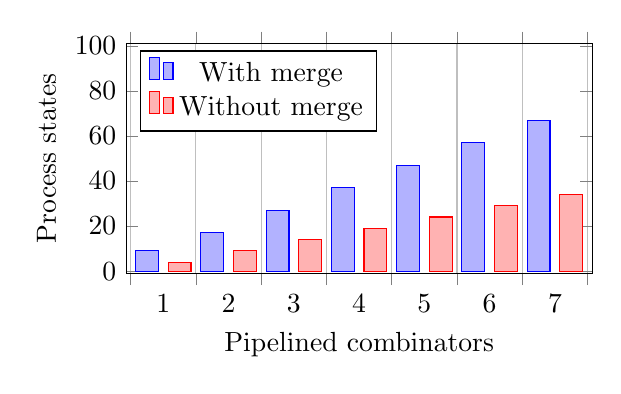
\begin{tikzpicture}
\begin{axis}[
% Hide the label on the second graph
	ylabel=Process states,
	xlabel=Pipelined combinators,
  ymin=0, ymax=100,
	enlargelimits=0.01,
	ybar interval=0.7,
  width=7.5cm, height=4.5cm,
	legend pos=north west,
]
\addplot coordinates {(1,9) (2,17) (3,27) (4,37) (5,47) (6,57) (7,67)   (8,1) };
\addplot coordinates {(1,4) (2,9) (3,14) (4,19) (5,24) (6,29) (7,34)    (8,1) };
\legend{With merge, Without merge};
\end{axis}
\end{tikzpicture}
\end{minipage}
\quad
\quad
\quad
\begin{minipage}[t]{0.4\textwidth}
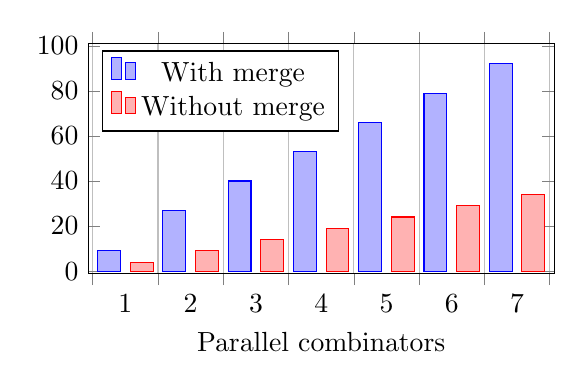
\begin{tikzpicture}
\begin{axis}[
%       ylabel=Process states,
        xlabel=Parallel combinators,
  ymin=0, ymax=100,
        enlargelimits=0.01,
        ybar interval=0.7,
  width=7.5cm, height=4.5cm,
        legend pos=north west,
]
\addplot coordinates {(1,9) (2,27) (3,40) (4,53) (5,66) (6,79) (7,92)
  % Last bar doesn't show for some reason, so need to add a dummy value for the next one
    (8,1) };

\addplot coordinates {(1,4) (2,9) (3,14) (4,19) (5,24) (6,29) (7,34)    (8,1) };

\legend{With merge, Without merge};
\end{axis}
\end{tikzpicture}
\end{minipage}

\caption{Maximum output process size for fusing all combinations of up to $n$ combinators.}
\label{fig:bench:outputsize}
\end{figure}


% -----------------------------------------------------------------------------
\begin{figure}

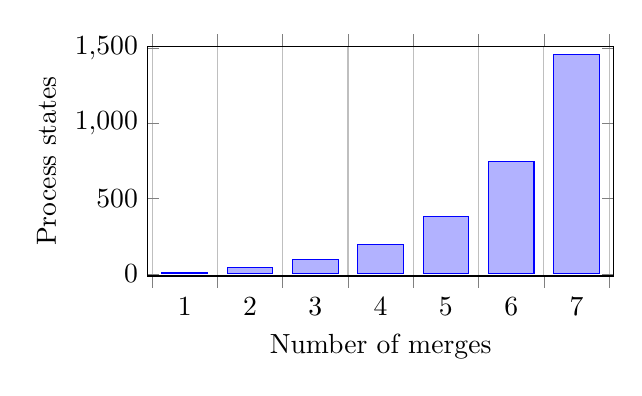
\begin{tikzpicture}
\begin{axis}[
	ylabel=Process states,
	xlabel=Number of merges,
%  ymode=log,
  ymin=0, ymax=1500,
	enlargelimits=0.01,
	ybar interval=0.7,
  width=7.5cm, height=4.5cm,
	legend pos=north west,
]
% These are the values for splitting.
% They are smaller than the 'chaining', but look much nicer on the linear graph.
\addplot coordinates {(1,9) (2,42) (3,97) (4,196) (5,383) (6,746) (7,1461)
  % (8,2880)
  (8,1)
  };

% These are the values for chaining
% \addplot coordinates {(1,4) (2,48) (3,194) (4,760) (5,2814) (6,10064) (7,1) };

\end{axis}
\end{tikzpicture}

\caption{Exponential blowup occurs when splitting or chaining merges together.}
\label{fig:bench:exponential}
\end{figure}

